
Um sinal � um conjunto de dados ou informa��es, que podem descrever diversos tipos de fen�menos, como um sinal de telefonia ou de voz (Figura \ref{fig:Voice}), o registro de vendas de uma empresa ou ainda os valores de fechamento de uma bolsa de valores (Figura \ref{fig:CotacaoBovespa}) \cite[p.~75]{Lathi}. Segundo \citeonline[p.~1]{Oppenheim} existe uma linguagem adequada para descrever sinais e um conjunto poderoso de ferramentas para analis�-los, capaz de se aplicar a problemas oriundos de diversos dom�nios. A s�rie de Fourier e a Transformada R�pida de Fourier s�o ambas exemplos destas ferramentas, e ser�o apresentadas nos pr�ximos cap�tulos.

\vspace{5.0mm}

\begin{figure}[H]
	\centering
	\captionsetup{width=0.8\textwidth, font=footnotesize, textfont=bf}	
	\includegraphics[width=0.8\linewidth]{Images/RevisaoDeLiteratura/CotacaoBovespa.png}
	\caption{�ndice BM \& FBOVESPA, S�o Paulo - Brasil}
	\vspace{-3.5mm}
	\caption*{Fonte: \citeonline{bovespa}}
	\label{fig:CotacaoBovespa}
\end{figure}

\vspace{4mm}

\begin{figure}[H]
	\centering
	\captionsetup{width=0.8\textwidth, font=footnotesize, textfont=bf}	
	\includegraphics[width=0.8\linewidth]{Images/RevisaoDeLiteratura/Voice.pdf}
	\caption{Sinal Refer�ncia de Voz}
	\vspace{-3.5mm}
	\caption*{Fonte: \citeonline{NirmalRaj}}
	\label{fig:Voice}
\end{figure}

\vspace{4mm}

\section{Sistemas de Tempo Continuo e Tempo Discreto}
	%\input{src/RevisaoDeLiteratura/STCTD.tex}

\section{S�rie de Fourier}
	
A s�rie de Fourier tem como principio os estudos das somas trigonom�tricas de senos e cossenos harmonicamente relacionados,  com o intuito de descrever fen�menos peri�dicos. Tal estudo possui uma longa hist�ria que data pelo menos da �poca dos babil�nicos, e que envolve  o estudo de diferentes fen�menos f�sicos. Mas o marco moderno neste tema ocorre em 1748 com o matem�tico e f�sico su��o Leonhard Paul Euler \cite[p.~104]{Oppenheim}. Euler em seu estudo sobre ondas estacion�rias atrav�s de cordas vibrantes observou que se a configura��o da posi��o vertical $y_0$ de um ponto horizontal $x$ em uma onda estacionaria  no tempo $t_0$ for uma combina��o linear dos modos normais da onda, o mesmo acontece com a configura��o em qualquer valor de tempo $t_s$ subsequente. Com base nesse estudo Euler demonstrou que � poss�vel calcular diretamente os coeficientes da combina��o linear em tempos futuros usando os coeficientes em tempos anteriores. \cite[p.~104]{Oppenheim}.  

\begin{figure}[H]
	\centering
	\captionsetup{width=0.7\textwidth, font=footnotesize, textfont=bf}	
	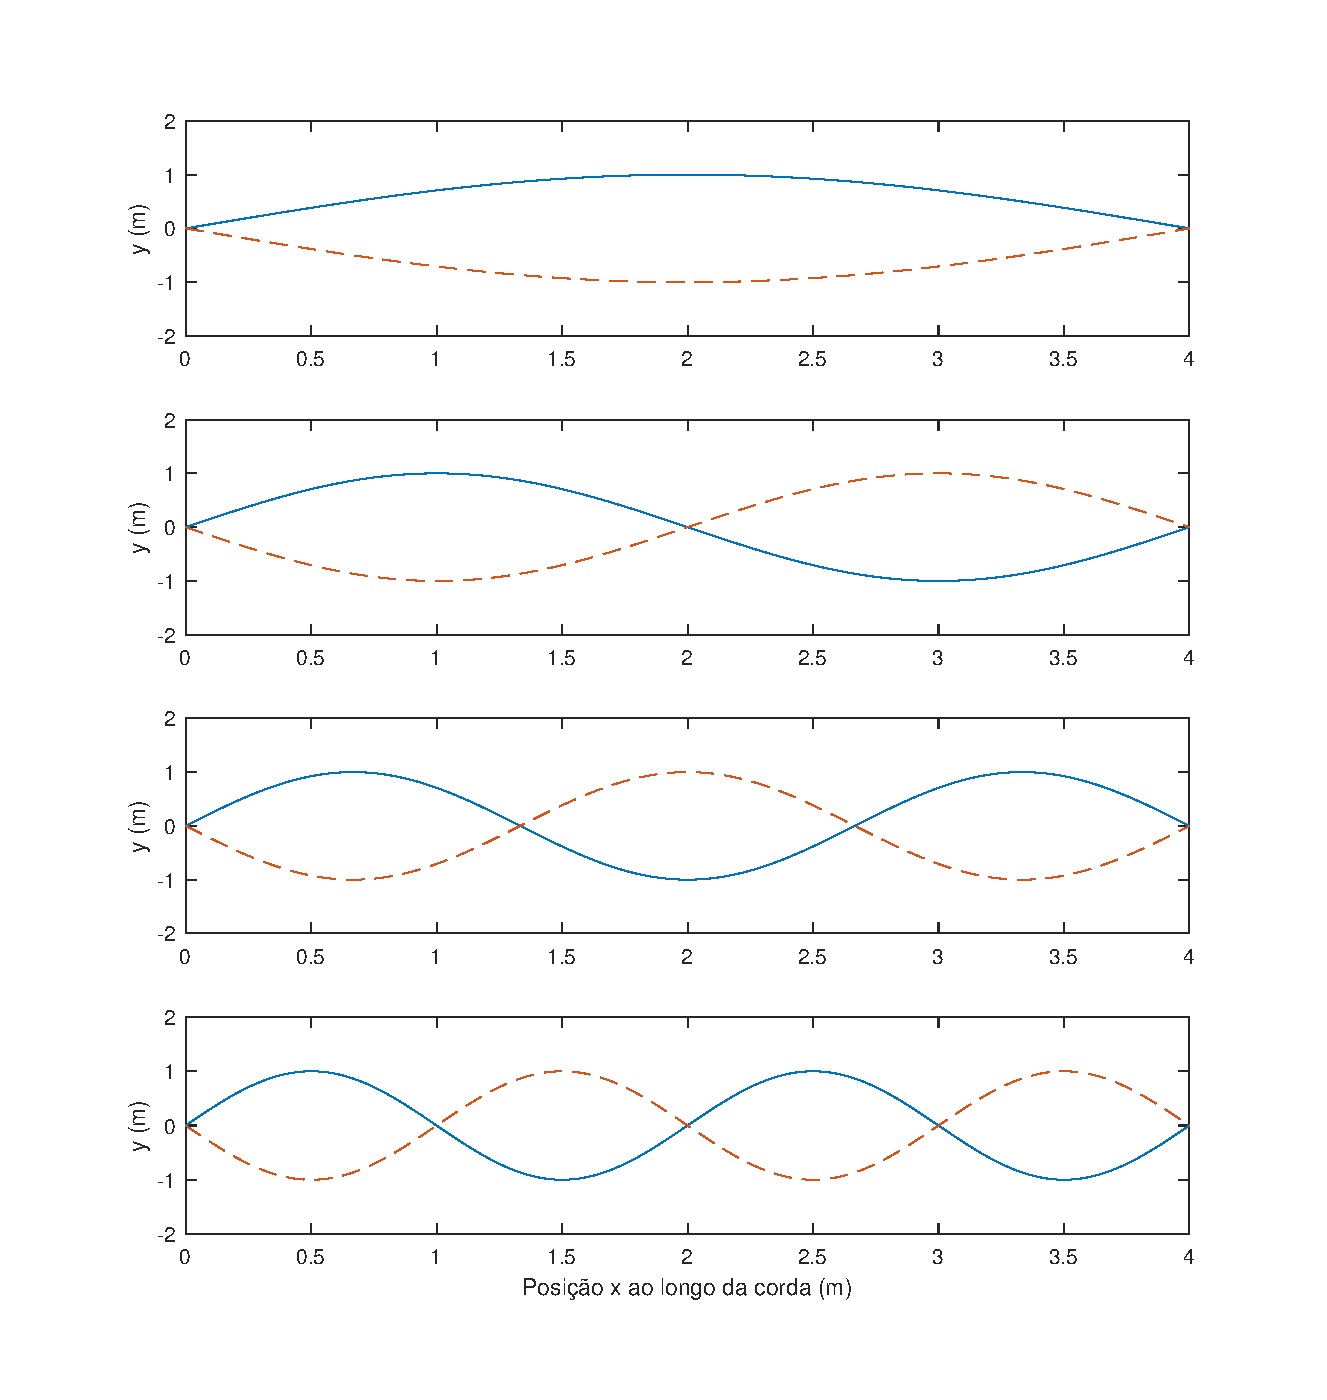
\includegraphics[width=0.7\linewidth]{Images/RevisaoDeLiteratura/OndasEstacionarias.eps}
	\caption{Modos Normais de uma Corda Vibrante}
	\vspace{-3.5mm}
	\caption*{Fonte: Adaptado de \citeonline[p.~105]{Oppenheim}}
	\label{fig:OndasEstacionarias}
\end{figure}


O estudo de Euler se tornam ainda mais importantes quando aplicado a sinas e a sistemas LIT. Segundo \citeonline[p.~163]{Haykin}, se a entrada de um sistema Linear Invariante no Tempo (LIT) for expressa por uma combina��o linear ponderada de sen�ides ou exponenciais complexas, a sa�da do sistema ser� expressa como uma combina��o linear ponderada da resposta do sistema a cada sen�ide ou exponencial complexa. Expressar sinais em termo de senoides ou exponenciais complexas n�o apenas leva a uma express�o alternativa �til para o comportamento da entrada e sa�da de um sistema LTI, como tamb�m fornece uma caracteriza��o muito criteriosa dos sinais e sistemas. O estudo de sinais e sistemas usando representa��o senoidal, ou exponencial complexa, � denominada an�lise de Fourier, em homenagem ao f�sico e matem�tico franc�s Jean-Baptiste Joseph Fourier (1768 - 1830) \cite[p.~163]{Haykin}.

Segundo \citeonline[p.~105]{Oppenheim}, meio s�culo depois da divulga��o do trabalho de Euler, Fourier havia se envolvido no estudo sobre s�ries trigonom�tricas, com a motiva��o f�sica de estudar o fen�meno da propaga��o e difus�o de calor. Fourier conclui que  s�ries senoidais harmonicamente relacionadas eram �teis na representa��o da distribui��o de temperatura em um corpo, e que 'qualquer' sinal peri�dico poderia ser representado po tal s�rie. Fourier ainda apresentou uma representa��o para sinais aperi�dicos, n�o atrav�s de somas ponderadas de senoides harmonicamente relacionadas, mas como integrais ponderadas de senoides que n�o s�o necessariamente harmonicamente relacionadas.

Como afirma \citeonline[p.~106]{Oppenheim}, muitas das ideias b�sica por tr�s das contribui��es de Fourier j� eram conhecidas, e as condi��es precisas sob as quais a representa��o de sinais proposta era v�lida s� foram apresentadas por P.L. Dirichlet em 1829. Por�m foi Fourier que que teve a clara percep��o do potencial pra essa representa��o, e at� certo ponto foi o seu trabalho e suas afirma��es que estimularam grande parte do trabalho subsequente. Logo em sua homenagem o estudo de sinais e sistemas, usando representa��es senoidais, � denominado an�lise de Fourier. E as s�ries pelo qual � realizada a representa��o de sinais na forma de somas de senoides complexas � doniminada s�rie de Fourier. 

\subsection{Resposta do Sistemas LTI a Entrada Senoidal} 

Na an�lise de Fourier, os sinais de entrada senoidais s�o comumente usados para caracterizar a resposta de um sistema LTI. A resposta senoidal em estado estacion�rio de um sistema LTI � obtido pela convolu��o entre a entrada senoidal e o sinal de impulso\cite[p.~163]{Haykin}. 

Ao aplicar um sinal impulso ($\delta (t)$) a entrada de um sistema LTI,  � gerado um sinal de sa�da, conhecido como resposta ao impulso $\delta (t)$. Atrav�s da resposta ao impulso � poss�vel caracterizar de maneira completa o comportamento de um sistema. A resposta ao impulso tamb�m possibilita conhecer a resposta do sistema LTI a qualquer sinal de entrada, atrav�s da convolu��o deste sinal ao impulso \cite[p.~108]{Haykin}.    

Assim realizando a convolu��o do impulso ao sinal senoidal, segundo \citeonline[p.~164]{Haykin}, a sa�da de um sistema LTI dado uma entrada senoidal complexa $x(t)$, na forma exponencial $e^(j \omega t)$, � dada por:

\begin{equation}
	y(t) = H(j \omega) e^{j \omega t}
	\label{eq:SaidaSenoideComplexa}
\end{equation}

Em que $H(j \omega)$ � a resposta em frequ�ncia, definida em termos de resposta ao impulso $delta (t)$. Assim;

\begin{equation}
	H(j \omega) = \int_{-\infty}^{\infty} \delta (t) e^{-j \omega t} dt
	\label{eq:RespostaSenoideComplexa}
\end{equation}

Logo a entrada senoidal complexa em um sistema LTI gera uma sa�da igual a entrada senoidal multiplicada apenas pela resposta em frequ�ncia do sistema $H(j \omega)$. 

As equa��es (\ref{eq:SaidaSenoideComplexa}) e (\ref{eq:RespostaSenoideComplexa}) apenas consideram como entrada um sinal senoidal. Por�m � de interesse obter uma express�o para a resposta do sistema LTI a quaisquer sinais arbitr�rios. Para tal \citeonline[p.~164]{Haykin} considera a senoide complexa $\psi~=~e^{j \omega t}$ como uma autofun��o do sistema $H$ associando com o autovalor $\lambda~=~H(j \omega)$, de modo a satisfazer:

\begin{equation}
	H\| \psi \| ~=~ \lambda \psi (t)
\end{equation}

Segundo \citeonline[p.~164]{Haykin} a sa�da do sistema dada a entrada de uma autofun��o � a dada pelo produto da entrada com um escalar. Esta rela��o pode ser vista na Figura (\ref{fig:PropriedadeDeAutofuncao}). 

\begin{figure}[H]
	\centering
	\captionsetup{width=0.7\textwidth, font=footnotesize, textfont=bf}	
	\includegraphics[width=0.7\linewidth]{Images/RevisaoDeLiteratura/PropriedadeDeAutofuncao.pdf}
	\caption{Ilustra��o da Propriedade de Autofun��o de Sistemas Lineares. (a) Autofun��o geral $\psi (t)$ e  autovalor $\lambda$. (b) Autofun��o senoidal complexa $e^{i \omega t}$ e autovalor $H(j \omega)$.}
	\vspace{-3.5mm}
	\caption*{Fonte: Adaptado de \citeonline[p.~164]{Haykin}}
	\label{fig:PropriedadeDeAutofuncao}
\end{figure} 
  

Segundo \citeonline[p.~530]{Lathi}  "Um sinal peri�dico $x(t)$ com per�odo $T_0$ pode
ser descrito como a soma de senoides de frequ�ncia $f_0$ e todas as suas harm�nicas", conforme visto em (\ref{eq:SerieFourierFundamental}). O qual e conhecida como s�rie trigonom�trica de Fourier de um sinal peri�dico $x(t)$, sendo $\omega_0$ a frequ�ncia fundamental.


\begin{equation}
	x(t) ~=~ a_0 + \sum _{n=1} ^{\infty} a_n cos (n \omega_0 t) + b_n sen(n \omega_0 t)
	\label{eq:SerieFourierFundamental}
\end{equation}

E poss�vel determinar os coeficientes $a_n$ e $b_n$ de (\ref{eq:SerieFourierFundamental} )pelas equa��es (\ref{eq:SerieFourierFundamentalan}) e (\ref{eq:SerieFourierFundamentalbn}), em que o coeficiente $T_0$ representa o per�odo relativo a $f_0$.

\begin{equation}
	a_n~=~\frac{2}{T_0} \int_{T_0} x(t) cos(n \omega_0 t) dt
	\label{eq:SerieFourierFundamentalan}
\end{equation}

\begin{equation}
	a_n~=~\frac{2}{T_0} \int_{T_0} x(t) cos(n \omega_0 t) dt
	\label{eq:SerieFourierFundamentalbn}
\end{equation}

A express�o da s�rie de Fourier em termos exponenciais $e^{j \omega_0 t}$ e $e^{?j \omega_0 t}$ � facilmente obtida a partir da forma trigonom�trica \cite{Lathi}. A forma exponencial da serie de Fourier � dada por (\ref{eq:SerieFourierExponencial}), em que o coeficiente $C_n$ e an�logo aos coeficientes $a_n$ e $b_n$ da serie trigonom�trica, sendo obtido por (\ref{eq:SerieFourierExponencialCn}.) Nota-se que diferente dos coeficientes $a_n$ e $b_n$, o coeficiente $C_n$ pode representar um valor complexo.

\begin{equation}
	x(t)~=~\sum^{\infty} _{- \infty} C_n e^{j n \omega_0 t}
	\label{eq:SerieFourierExponencial}
\end{equation}

\begin{equation}
	C_n~=~ \frac{1}{T_0} \int_{T_0} x(t) e^{j n \omega_0 t} dt
	\label{eq:SerieFourierExponencialCn}
\end{equation}

\subsection{Espectro Exponencial de Fourier}

Segundo \citeonline[p.~556]{Lathi}, o espectro exponencial de Fourier e tra�ado a partir dos coeficientes $C_n$ e das frequ�ncias $n \omega_0$ da forma exponencial da serie de Fourier. Ent�o e necess�rio expressar o espectro em fun��o da parte real e da parte imaginaria, ou do modulo e do �ngulo. A forma de $C_n$ em modulo � angulo geralmente � mais �til para se expressar o espectro. Logo s�o ta�ados dois gr�ficos para o espectro exponencial de Fourier, um que relaciona $|C_n |$ com $n \omega_0$, e outro que relaciona $\angle C_n$ com $n \omega_0$.

Para \citeonline[p.~533]{Lathi} os dois gr�ficos juntos formam o espectro de frequ�ncia, o qual revela os conte�dos de frequ�ncia do sinal $x(t)$, com suas
amplitudes e fase. Conhecendo-se este espectro n�o s� � poss�vel analisar o sinal
$x(t)$, como tamb�m reconstru�-lo de forma f�cil.

	
\section{S�rie de Fourier em Tempo Discreto}
	Ate aqui foi apresentada a forma continua da s�rie de Fourier, por�m para ser �til em uma aplica��o computacional � necess�rio encontrar sua forma discreta, ou DFT \textit{(Discrete Fourier Transform)}. Segundo \citeonline[p.~314]{Haykin} a DFT � a �nica representa��o de Fourier que pode ser calculada por um computador, sendo amplamente usada para manipular sinais.

O primeiro passo para se obter uma DFT e considerar o teorema da Amostragem. Tal teorema afirma que um sinal real $x(t)$, cujo o espectro e limitado em $\phi~Hz$, pode ser reconstru�do a partir de suas amostras tomadas uniformemente a uma taxa $f_s \textgreater 2 \phi$ \cite[p.~679]{Lathi}. Em seguida, a amostragem de $x(t)$, feita a
uma frequ�ncia $f_s$, pode ser obtida pela multiplica��o de $x(t)$ por um trem de impulsos $\delta (t)$. Sendo tais impulsos unit�rios e peri�dicos, repetidos a cada  $T~=~1/f_s$ segundos, por um numero total de amostras $N_0$, a amostragem pode ser definida por:

\begin{equation}
	\overline{x}(t)~=~x(t) \delta_{T}(t)~=~\sum^{N_0 -1} _{n=0} x(nT) \delta(t-nT)
	\label{eq:FourierAmostragem}
\end{equation}

Por conveni�ncia, deseja-se obter um espectro do sinal amostrado $x(t)$ em fun��o de $\omega$ ou expresso em termos de frequ�ncia. Para tal, segundo \citeonline[p.~681]{Lathi}, o trem de impulsos $\delta(t)$ e um sinal peri�dico que pode ser descrito pela s�rie trigonom�trica de Fourier da seguinte forma:

\begin{equation}
	\delta_T (t)~=~\frac{1}{T} [1+ 2cos(\omega_s t) + 2cos(2\omega_s t) + 2cos(3\omega_s t) + \dotsc]
	\label{eq:TremDeImpulsos}
\end{equation}

Logo, multiplicando $x(t)$ por $\delta_{T} (t)$, obt�m-se:

\begin{equation}
	\overline{x}(t)~=~x(t) \delta_{T}(t)~=~\frac{1}{T} [x(t) + 2x(t)cos(\omega_s t) + 2x(t)cos(2 \omega_s t) + 2x(t)cos(3 \omega_s t) + \dotsc]
	\label{eq:FourierAmostragemTremDeImpulsos}
\end{equation} ?

Segundo \citeonline[p.~125]{Oppenheim}, a transformada de Fourier do primeiro termo $x(t)$, em (\ref{eq:FourierAmostragemTremDeImpulsos}), � $X(\omega)$. J� a transformada de Fourier do segundo termo 2x(t)cos(!st) � $X(\omega ? \omega_s)~+~X(\omega + \omega_s)$, e do terceiro termo $2x(t)cos(2 \omega_s t)$ �
$X(\omega ? 2 \omega_s) + X(\omega + 2 \omega_s)$. E assim, semelhantemente a transformada de Fourier dos demais termos da serie que descreve (\ref{eq:FourierAmostragemTremDeImpulsos}), representam o espectro $X(\omega)$ deslocado em $n\omega_s$ e $?n\omega_s$. Assim,

\begin{equation}
	\overline{X}( \omega )~=~ \frac{1}{T} \sum_{\infty}^{-\infty} X(\omega - n \omega_s)
	\label{eq:FourierAmostragemDeslocada}
\end{equation}

Desde que a frequ�ncia de amostragem $f_s$ garanta o crit�rio do teorema da Amostragem, o sinal $\overline{X}$ ser� constitu�do de repeti��es n�o sobrepostas de $x(\omega_0)$, a um intervalo de tempo $T = 1/f_s$. Logo tanto $\overline{X}(\omega)$, quanto $\overline{x}(t)$ s�o peri�dicas e equivalentes, por�m com representa��es distintas do especto amostrado. Sendo assim, atrav�s da propriedade de deslocamento no tempo da transformada de Fourier (\ref{eq:Impulso}) e da e (\ref{eq:FourierAmostragem}), obt�m-se (\ref{eq:FourierAmostragemExponencial}) \citeonline[p.~125]{Oppenheim}:

\begin{equation}
	\delta(t - nT) \longleftrightarrow e^{-jn \omega T }
	\label{eq:Impulso}
\end{equation}

\begin{equation}
	\overline{x}(t)~=~\sum_{n=0}^{N_0 - 1} x(nT)e^{-j n \omega T}
	\label{eq:FourierAmostragemExponencial}
\end{equation}

Segundo \citeonline[p.~705]{Lathi}, a transformada de $\overline{x}(t)$ pode ser aproximada, considerando um certo \textit{aliasing} negligenci�vel, para $X(\omega)/T$. Portanto:

\begin{equation}	
	X(\omega)~=~T \sum_{n=0}^{N_0 - 1} x(nT) e^{j n \omega T} ~~ |\omega| \leq \frac{\omega_s}{2}
	\label{eq:DefinicaoDFT}	
\end{equation}

Analisando a propriedade peri�dica de $x(t)$ e $X(\omega)$, e considerando $x(nT)$ e $X(r\omega_0)$ a n-�sima e r-�sina amostra de $x(t)$ e $X(\omega)$, respectivamente, s�o definidas as seguintes vari�veis:

\begin{equation}
	x_n~=~Tx(nT)
	\label{eq:DefinicaoDFTA}
\end{equation}

\begin{equation}
	x_n~=~\frac{T_0}{N_0}x(nT)
	\label{eq:DefinicaoDFTB}
\end{equation}

\begin{equation}
	X_r ~=~ X ( \omega )
	\label{eq:DefinicaoDFTC}
\end{equation}

\begin{equation}
	\omega~=~r \omega_0
	\label{eq:DefinicaoDFTD}
\end{equation}

\begin{equation}
	X_r~=~X(r \omega_0)
	\label{eq:DefinicaoDFTE}
\end{equation}

\begin{equation}
	\omega_0~=~2 \pi f_0 ~=~\frac{2 \pi}{T_0}
	\label{eq:DefinicaoDFTF}
\end{equation}

Assim, substituindo (\ref{eq:DefinicaoDFTE}) e (\ref{eq:DefinicaoDFTB}) em (\ref{eq:DefinicaoDFT}), e fazendo $\omega_0 T = \Omega_0 = 2 pi /N_0$, se
obt�m a seguinte express�o para a transformada discreta de Fourier \cite[p.~125]{Oppenheim}:

\begin{equation}
	X_r~=~\sum_{n=0}^{N_0 - 1} x_n e^{j \omega_0 n r}
	\label{eq:DefinicaoDFTG}
\end{equation}

Onde:

\begin{equation}
	\Omega_0~=~\frac{2 \pi}{N_0}
	\label{eq:DefinicaoOmega}
\end{equation}

Para compactar a express�o de (\ref{eq:DefinicaoDFTG}) se faz a substitui��o da express�o exponencial pela vari�vel  $W$, de modo que $W_{N_0} = e^{?2 \pi /N_0} = e^{-j \Omega_0}$. Logo a express�o para DFT � dada por (\ref{eq:DFT}) \cite[p.~344]{Meyer}:

\begin{equation}
	X_r~=~\sum_{n=0}^{N_0 - 1} x_n e^{j \omega_0 n r}
	\label{eq:DFT}
\end{equation}

Onde:

\begin{equation}
	0 \leq k  \leq N_0 - 1
	\label{eq:N0}
\end{equation}


	
\section{Transformada R�pida de Fourier}
	
Para se calcular uma DFT de $N_0$ valores usando apenas (\ref{eq:DFT}), e necess�rio realizar um total de $N^2_0$ multiplica��es e  $N_0(N0 ? 1)$ somas utilizando n�meros complexos. Deste modo, quando $N_0$ assume um valor elevado, muitos recursos computacionais s�o necess�rios, at� chegar ao ponto de que esse algoritmo se torna impratic�vel.

Para que se possa reduzir o numero de opera��es matem�ticas necess�rias para calcular a DFT � que surgiu o algoritmo criado por J.W. Cooley e John Tukey, conhecido como Transformada R�pida de Fourier ou FFT \textit{(Fast Fourier Transform)} \citeonline[p.~719]{Lathi}. Para reduzir o numero de c�lculos, a FFT se utiliza da propriedade linear da transformada de Fourier. J� que, segundo \citeonline[p.~119]{Oppenheim}, a transformada de Fourier de um sinal pode ser dada pela combina��o linear da transformada de Fourier de segmentos menores do mesmo sinal. Logo, � poss�vel aplicar a DFT o paradigma da Divis�o e Conquista, o qual � um recurso muito utilizado em algoritmos de ordena��o. 

Segundo \citeonline[p.~21]{cormen} um algoritmo de Divis�o e Conquista realiza o desmembramento de um problema em v�rios subproblemas que s�o id�nticos ao original, por�m menores em sua faixa de a��o, o que os torna mais simples de resolver. Em seguida, resolvem-se os subproblemas recursivamente e combinam-se essas solu��es de modo a obter a solu��o para o problema original.

De modo muito semelhante o algoritmo da FFT prev� uma divis�o recursiva  da DFT em dois blocos: bloco par e o bloco �mpar, como mostrado em (\ref{eq:DenicaoFFT}) \cite[p.~35]{chu}. Nesta mesma equa��o os limites dos somat�rios de ambas as parcelas �mpar e par foram redefinidas para englobar apenas metade dos $N_0$ pontos, bem como os expoentes de $W$ foram ajustados.

\begin{equation}
	X_r~=~\underbrace{\sum^{\frac{N_0}{2} - 1}_{n=0} x_{2n} W^{2nr}_{N_0}}_{Parcela~Par} ~ + ~\underbrace{\sum^{\frac{N_0}{2} - 1}_{n=0} x_{2n+1} W^{(2n+1)r}_{N_0}}_{Parcela~\acute{I}mpar}
	\label{eq:DenicaoFFT}  
\end{equation}

Utilizando algumas das propriedades geom�tricas de $W$, j� que o mesmo representa um numero complexo, pode-se realizar simplifica��es importantes em \ref{eq:DenicaoFFTA}. Primeiro nota-se que $W_{N_0 / 2}~=~W_{N_0} ^{2}$, logo:

\begin{equation}
	X_r~=~\underbrace{\sum^{\frac{N_0}{2} - 1}_{n=0} x_{2n} W^{2nr}_{N_0}}_{G_r} ~ + ~\underbrace{\sum^{\frac{N_0}{2} - 1}_{n=0} x_{2n+1} W^{(2n+1)r}_{N_0}}_{H_r}
	\label{eq:DenicaoFFTA}  
\end{equation}

Como $G_r$ e $H_r$ s�o DFTs com $N_0 / 2$ pontos cada, ent�o ambos possuem um per�odo de $N_0 / 2$. Com base na propriedade peri�dica destas DFTs pode-se utilizar as simplifica��es (25) e (26) para reduzir o n�mero de c�lculos na DFT \cite[p. 721]{Lathi}.


	
\section{FPGA}
	\citeonline[p.~4]{Moore} define a FPGA como um dispositivo semicondutor capaz de ser totalmente redefinido ap�s sua fabrica��o, permitindo ao programador reconfigurar produtos e fun��es j� implementadas, adaptando o \emph{hardware} a novas fun��es. De forma pr�tica, a FPGA permite uma flexibilidade em um projeto, podendo mudar a forma como ele � implementado, sem a necessidade de se construir um \emph{hardware} novo. 

Para \citeonline[p.~4]{Moore}, comparado com as outras formas de construir um hardware, a FPGA oferece duas grandes vantagens em uma aplica��o. Primeiro, para uma aplica��o ao inv�s de se utilizar um circuito integrado padr�o comercial, que geralmente �  super ou subdimensionado, ou ainda desenvolver um novo projeto de circuito integrado especifico, consumindo tempo e recursos, a FPGA  possibilita desenvolver um \textit{hardware} exatamente dentro das especifica��es, personalizado e otimizado para a fun��o destinada. Em segundo, por�m t�o importante quanto, � que essa capacidade de personaliza��o de \textit{hardware} possibilita a realiza��o de opera��es de modo mais simplificado, r�pido e energeticamente eficiente se comparado a um microprocessador.

\subsection{Aspectos Construtivos da FPGA}

As FPGAs s�o baseadas em unidades l�gicas elementares b�sicas, ou BLEs (\textit{Basic Logic Elements}), dentro de uma hierarquia de interconex�es reconfigur�veis que permitem que os LEs sejam fisicamente conectados uns aos outros de diferentes formas criando uma enorme variedade de componentes digitais. A arquitetura das FPGAs modernas s�o constitu�das basicamente por conjunto de mem�rias de armazenamento em massa SRAM (\textit{Static Random Access Memory}), Portas de Entrada/Sa�da, blocos l�gicos configur�veis CLB (\textit{Configurable Logic Blocks}) e sistema de roteamento, como pode ser visto na Figura (\ref{fig:FPGAArchitecture}) \cite[p.~5]{Moore}. 

\vspace{8mm}
\begin{figure}[H]
	\centering
	\captionsetup{width=0.5\textwidth, font=footnotesize, textfont=bf}	
	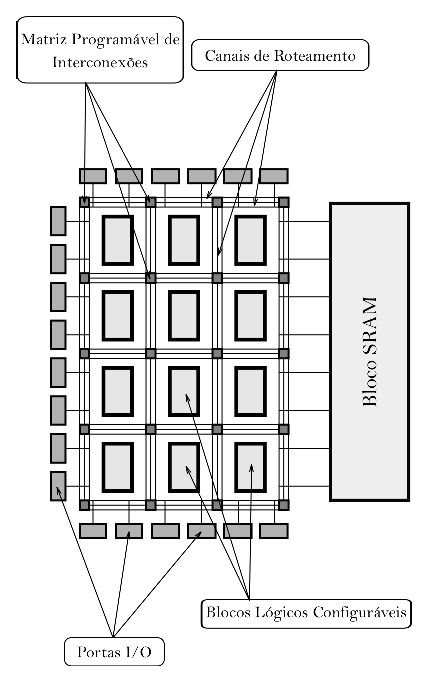
\includegraphics[width=0.5\linewidth]{Images/RevisaoDeLiteratura/FPGAArchitecture.eps}
	\caption{Arquitetura Tipica de uma FPGA}
	\vspace{-3.5mm}
	\caption*{Fonte: Adaptado \citeonline[p.~6]{Meyer}}
	\label{fig:FPGAArchitecture}
\end{figure}
\vspace{8mm}

Os  CLB s�o blocos realizam opera��es logicas b�sicas e armazenam pequenos volumes de dados. Comumente as opera��es complexas, necess�rias para o processamento de uma aplica��o, s�o divididas em processos mais simples para cada uma das CLBs selecionadas, de modo que a soma das tarefas de cada CLB seja equivalente a opera��o complexa, em uma estrat�gia de divis�o e conquista. Para realizar opera��es l�gicas b�sicas e ainda armazenar pequenos volumes de dados os CLBs tecnicamente poderiam ser apenas um pequeno circuito de transistores (granularidade fina), ou at� mesmo um processador completo (granularidade grosseira). Se os CLBs fossem granularidade fina, para realizar tarefas complexas seria necess�rio um grande n�mero de CLBs e um sistema de roteamento complexo para interconecta-los, o que resultaria em uma FPGA de baixa performance e um elevado consumo energ�tico. Por outro lado de as CLBs forem de uma granularidade mais grosseira seria um desperd�cio de recurso utiliza-los em opera��es mais simples \cite[p.~11]{tree}. Assim a escolha do n�vel de complexabilidade, ou granula��o, das CLBs de uma FPGA � um compromisso de otimiza��o de recursos.

Ainda segundo \citeonline[p.~11]{tree} dentro da grama de granula��o das CLBs, algumas arquiteturas incluem o uso de portas NAND, interconex�o de multiplexadores e tabelas de busca LUT (\textit{Lookup Table}). Em especial fabricantes como a Xilinx utilizam CLBs baseadas em LUTs, j� que CLBs baseadas em LUT oferecem uma boa rela��o de granula��o, otimizando os recursos da FPGA para aplica��es simples at� as mais complexas. Este tipo de CLB  pode incluir uma �nico elemento logico b�sico BLE (\textit{Basic Logic Element}), ou mesmo um \textit{cluster} de BLEs interconectados, como mostrado na Figura (\ref{fig:ArchitectureClusterBLE}).

\vspace{6mm}
\begin{figure}[H]
	\centering
	\captionsetup{width=0.4\textwidth, font=footnotesize, textfont=bf}	
	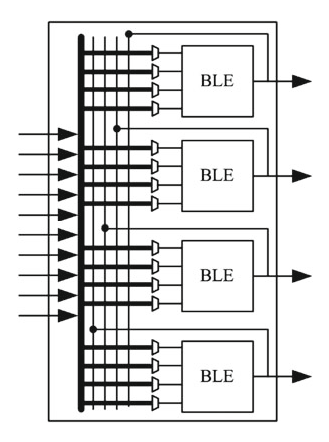
\includegraphics[width=0.4\linewidth]{Images/RevisaoDeLiteratura/ArchitectureClusterBLE.eps}
	\caption{Arquitetura de uma CLB com 4 BLEs}
	\vspace{-3.5mm}
	\caption*{Fonte: Adaptado \citeonline[p.~13]{tree}}
	\label{fig:ArchitectureClusterBLE}
\end{figure}
\vspace{6mm}

Segundo \citeonline[p.~11]{tree}, um BLE mais simples consiste basicamente de um LUT e um \textit{Flip-Flop} tipo D, como pode ser visto na Figura (\ref{fig:BasicLogicElement}). Um LUT com $k$ entradas pode implementar $k$ fun��es booleanas utilizando os espa�os de mem�ria SRAM dentro da LUT. O exemplo apresentado na Figura (\ref{fig:BasicLogicElement}) utiliza  16 bits de mem�ria SRAM, os quais s�o conectadas a entrada do multiplexador que possui 4 bits de sele��o, e cuja sa�da � ligada ao \textit{flip-flop}. Esta configura��o permite que a LUT tenha $2^k$ combina��es das $k$ opera��es booleanas. 

\vspace{6mm}
\begin{figure}[H]
	\centering
	\captionsetup{width=0.5\textwidth, font=footnotesize, textfont=bf}	
	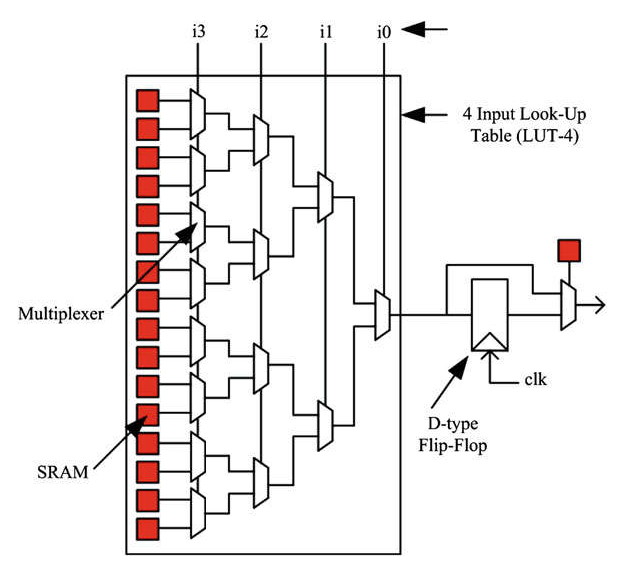
\includegraphics[width=0.5\linewidth]{Images/RevisaoDeLiteratura/BasicLogicElement.eps}
	\caption{Arquitetura de uma BLE (\textit{Basic Logic Element})}
	\vspace{-3.5mm}
	\caption*{Fonte: Adaptado \citeonline[p.~13]{tree}}
	\label{fig:BasicLogicElement}
\end{figure}
\vspace{6mm}

Um �nico BLE � capaz de realizar algumas opera��es booleanas b�sicas, por�m em clusters as combina��es de opera��es aumentam. FPGAs modernas tipicamente cont�m de 4 a 10 BLEs em um �nico cluster. Por�m estas FPGAs n�o possui apenas BLEs id�nticas, na verdade h� uma grande heterogenia de blocos, sendo muitos deles desenvolvidos para prop�sitos espec�ficos. Entre estes blocos de prop�sito espec�fico est�o multiplicadores, somadores, mem�rias e DSPs (\textit{Digital Signal Processor}), entre outros. Estes blocos s�o desenvolvidos para otimizar o espa�o, processamento, roteamento e demais recursos de \textit{hardware} que seriam necess�rios para implementar as mesmas fun��es em BLEs comuns, sendo essenciais em certas aplica��es \citeonline[p.~10]{tree}.

A implementa��o de qualquer circuito l�gico � feita pela associa��o de diferentes blocos l�gicos e pelas portas de entrada e sa�da da FPGA, os quais s�o conectados uns aos outros atrav�s da rede de roteamento program�vel, ou PLN (\textit{Programmable Logic Network}). Na Figura (\ref{fig:FPGAArchitecture}) a PLN � representada pela Matriz Program�vel de Interconex�es e pelos Canais de Roteamento. Para que a FPGA possa implementar qualquer circuito digital as interconex�es de roteamento devem ser flex�veis para suportar a grande variedade de conex�es demandada, otimizando sempre as dist�ncias das conex�es e reduzindo a lat�ncia dos sinais.  Portanto ao projetar um circuito a ser implementado na FPGA deve ser ter especial aten��o a forma como o roteamento do blocos l�gicos � feito, buscando flexibilidade e efici�ncia \citeonline[p.~13]{tree}.

Nas FPGAs modernas al�m da unidades de armazenamento de Dados SRAM contido dentro das BLEs, mais especificamente nas LUTs, existe ainda grandes blocos SRAM isolados das BLEs, destinados a funcionar como o armazenamento de dados em massa. Estes blocos s�o importantes em aplica��es digitais onde  � necess�rio armazenar, como por exemplo, dados de amostragem ou mesmo dados p�s-processamento que devem aguardar para serem passados para uma pr�xima etapa de processamento, ou mesmo transmitidos para fora da FPGA pelas portas de entrada e sa�da de dados. Estes bloco de mem�ria � apresentada na Figura (\ref{fig:FPGAArchitecture}) como parte integrante da arquitetura tipica de uma FPGA.

\subsection{Programa��o na FPGA}

O desenvolvimento de uma aplica��o em FPGA come�a pela elabora��o do Design de Refer�ncia, que nada mais � do que uma descri��o l�gica equivalente que deve ser programada na FPGA para implementa��o das opera��es l�gicas desejadas. O Design de Refer�ncia pode ser feito utilizando diagrama de portas l�gicas ou ainda usando qualquer linguagem de descri��o de hardware como VHDL (\textit{VHSIC Hardware Description Language}) ou Verilog. A maioria dos ambientes de desenvolvimento integrados (IDE - \textit{Integrated Development Environment}), disponibilizados pelos fabricantes de FPGAs possuem  a op��o de programa��o visual utilizando portas l�gicas. A Figura (\ref{fig:ExemploFullAdder4Bits}) apresenta o diagrama de um somador de 4 bits, feito no IDE ISE Design Suite 14, da fabricante Xilinx. 

\vspace{6mm}
\begin{figure}[H]
	\centering
	\captionsetup{width=\textwidth, font=footnotesize, textfont=bf}	
	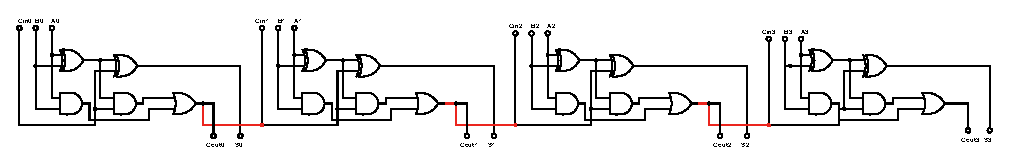
\includegraphics[width=\linewidth]{Images/RevisaoDeLiteratura/ExemploFullAdder4Bits.eps}
	\caption{Diagrama L�gico Full Adder 4 Bits - ISE Design Suite 14}
	\vspace{-3.5mm}
	\caption*{Fonte: Autoria Pr�pria}
	\label{fig:ExemploFullAdder4Bits}
\end{figure}
\vspace{6mm}

Programar um somador de 4 bits como apresentado na Figura (\ref{fig:ExemploFullAdder4Bits}), utilizando portas l�gicas parece ser realmente simples. Por�m para circuitos mais elaborados como um contador, ou at� mesmo uma m�quina de estados, pode ser tornar impratic�vel utilizar este m�todo de desenvolvimento. Pra circuitos mais elaborados � poss�vel utilizar uma linguagem de descri��o de \textit{hardware} HDL (\textit{Hardware Description Linguage}), para tornam o desenvolvimento mais f�cil e intuitivo. Tendo em vista ainda que uma linguagem descritiva, como por exemplo VHDL, � visivelmente mais familiar ao desenvolvedor que est� acostumado a linguagens de programa��o como por exemplo Linguagem C. O C�digo (\ref{code:ExemploFullAdder4Bits}) descrito abaixo apresenta o mesmo somador de 4 bits desenvolvido em VHDL. 

\vspace{3mm}
	\lstset{style=VHDL}
	\begin{lstlisting}
	library IEEE;
	use IEEE.STD_LOGIC_1164.ALL;
	use IEEE.NUMERIC_STD.ALL;
	
	entity FullAdder4Bits is
		port(InputA : in unsigned(3 downto 0);
		 InputB : in unsigned(3 downto 0); 
		 Result : out unsigned(3 downto 0); 
		 CarryOut : out std_logic);
	end entity;
	
	architecture Behavioral of FullAdder4Bits is
		
		signal Aux : unsigned(4 downto 0);
		
	begin 
		
		Aux <= ("0" & InputA) + InputB; 
		Result <= temp(3 downto 0); 
		CarryOut <= Aux(4);
		
	end architecture Behavioral;
	\end{lstlisting}
	\label{code:ExemploFullAdder4Bits}
\vspace{3mm}

Ap�s definir o Design de Refer�ncia, via diagrama de portas l�gicas ou mesmo por c�digo HDL, o pr�ximo passo � utilizar uma ferramenta de s�ntese da pr�pria IDE para converter o design de refer�ncia em um conjunto de configura��es de registradores, conex�es e portas que ser�o usadas  na FPGA para implementar as funcionalidades descritas no designe de refer�ncia. Durante o processo de s�ntese a ferramenta verifica a sintaxe do c�digo HDL, e a coer�ncia entre as portas de externas, como sinais de \textit{clock} e portas de entrada e sa�da,  selecionadas no design de refer�ncia.

Ao desenvolver um design para implementa��o em FPGA � comum dividir as funcionalidades do sistema em pequenos blocos de modo a modulariza-lo, permitindo reaproveitar trechos de circuitos l�gicos em diferentes aplica��es. Segundo \citeonline[p.~20]{Moore} ao longo dos anos os fabricantes FPGA perceberam tamb�m que v�rios dos sistemas implementados pelos desenvolvedores tinham funcionalidades muito comuns, como por exemplo processamento gr�fico, interfaces de comunica��o serial e at� mesmo implementa��o de microprocessadores. Logo n�o fazia sentido o desenvolvedor desperdi�as tempo implementando um circuito extremamente comum. Assim os fabricantes passaram a oferecer bibliotecas circuitos l�gicos modularizados para funcionalidades comuns, que passaram a ser chamados de IP (\textit{Intellectual Property}).
 
A maioria dos IDEs mais recentes possuem uma interface gr�fica de diagrama de blocos, onde cada bloco representa uma IP. Nesta interface � poss�vel construir um Design de Refer�ncia utilizando a associa��o de IPs das bibliotecas do fabricante, ou de um reposit�rio externo ou ainda utilizar uma IP pr�pria, j� que estes IDEs possibilitam a cria��o de IPs personalizadas. A Figura (\ref{fig:ExemploDiagramaDeBlocosMicroBlazeUART}) apresenta o diagrama de blocos de um circuito l�gico desenvolvido na IDE Vivado 2017.4, composto pelas seguintes IPs da Biblioteca padr�o Xilinx: microprocessador MicroBlaze 10.0, bloco seu mem�ria local, o controlador de perif�ricos MicroBlaze, a interface de comunica��o UART, controle global de interrup��es e controle de global de reset. E ainda IP \textit{FFT16p\_V1\_0\_0} desenvolvida individualmente utilizando c�digo VHDL.

\vspace{6mm}
\begin{figure}[H]
	\centering
	\captionsetup{width=\textwidth, font=footnotesize, textfont=bf}	
	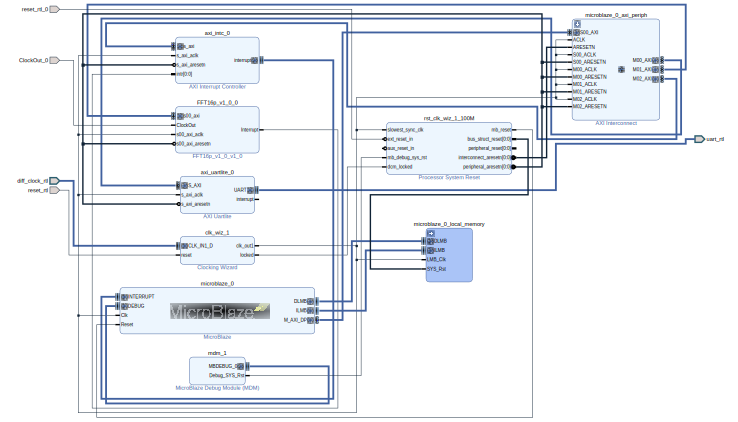
\includegraphics[width=\linewidth]{Images/RevisaoDeLiteratura/ExemploDiagramaDeBlocosMicroBlazeUART.png}
	\caption{CPU MicroBlaze e Coprocessador para FFT com Interface UART - Vivado 2017.4}
	\vspace{-3.5mm}
	\caption*{Fonte: Autoria Pr�pria}
	\label{fig:ExemploDiagramaDeBlocosMicroBlazeUART}
\end{figure}
\vspace{6mm}
 
A FPGA � uma boa escolha para a implementa��o do algoritmo da FFT  devido a grande variedade de recursos de hardware sintetiz�veis, al�m de possuir recursos de programa��o paralela que permite o processamento paralelo de sinais, conferindo assim uma maior rapidez na execu��o do algoritmo \cite{kamal}. Como afirma \citeonline[Pref�cio]{Meyer}, muitos algoritmos de processamento de sinais, como FFT (\emph{Fast Fourier Transform}) e os filtros FIR ou IIR,  implementados anteriormente em Circuitos Integrados de Aplica��o Especifica ou ASIC (\emph{Application Specific Integrated Circuits}), agora est�o sendo implementados em FPGAs.



\subsection{ZynqBerry TE0726-03M}

O dispositivo escolhido para a implementa��o do algoritmo Radix-2 � o  \textit{ZynqBerry - TE0726} da fabricante \textit{Trenz Eletronic$^\circledR$}, apresentado na figura (\ref{fig:ZynqBerry-TE0726}). Este dispositivo � baseado no SoC (\textit{System On Chip}) Raspberry Pi modelo 2, vem equipado com uma FPGA SoM (\textit{System on Module}) XC7Z010-1CLG225C-REV3, da fam�lia Zynq-700 fabricado pela \textit{Xilinx$^\circledR$} \cite{trenz}. 

\vspace{6mm}
\begin{figure}[H]
	\centering
	\captionsetup{width=0.6\textwidth, font=footnotesize, textfont=bf}	
	\includegraphics[width=0.6\linewidth]{Images/RevisaoDeLiteratura/TE0726-03M_0.jpg}
	\caption{ZynqBery - TE0726}
	\vspace{-3.5mm}
	\caption*{Fonte: \citeonline{trenz}}
	\label{fig:ZynqBerry-TE0726}
\end{figure}
\vspace{6mm}


A FPGA XC7Z010-1CLG225C tem a mesma arquitetura dos modelos da fam�lia Artix-7, tamb�m da Xilinx, e contendo recursos como: 28.000 c�lulas l�gicas, 17.600 LUTs, 2.1 Mb de mem�ria RAM divididos em blocos de 26Kb e um total de 36.200 \textit{flip-flops}. Cada CLB, nesta FPGA, para implementar diferentes opera��es l�gicas utiliza 16 \textit{flip-flops}, 2 somadores de 4bits cascate�veis e ainda 8 LUTs. Sendo poss�vel configurar a memoria RAM das LUTs para 64x1 ou 32x2 bits, ou ainda como um  \textit{shift register (SRL)}. Al�m disso esta FPGA possuir 80 blocos DSP, cada um equipado com um multiplicador 18x25 simples, e um somador/acumulador de 48 bits. Todas estes recursos fazem do XC7Z010 um \textit{hardware} competente para as mais diversas aplica��es de processamento de sinais, como o calculo da FFT.

O processador utilizado no ZynqBerry TE0726-03M � um dual-core ARM Cortex-A9 de 866MHz � competente na execu��o eficiente de sistemas operacionais completos como o sistemas baseados em kernel Linux, que podem incluem interface gr�fica sofistica. Cada n�cleo deste processador conta ainda uma unidade NEON\texttrademark  Media Processing Engine (MPE), para alto desempenho em codifica��o e decodifica��o de �udio e v�deo, e uma unidade de ponto flutuante para incremento da precis�o em opera��es matem�ticas.  Aliando a versatilidade da XC7Z010 e o poder de processamento do ARM Cortex-A9 � poss�vel construir dispositivo que rode uma vers�o Linux, tirando proveito de toda a funcionalidade de tal sistema operacional pode prover, e que ainda disponha de um \textit{hardware} acelerador personalizado para uma aplica��o especifica, e que trabalhe em paralelo � uma alta frequ�ncia. Provendo assim uma solu��o engenhosa de alto desempenho para processamento de sinais.


\subsubsection{Zynq-7000}

Segundo a \citeonline{zynqbook}, Zynq-7000 � uma fam�lia de SoCs que integram a programabilidade em \textit{software} de um processador ARM  Cortex-A9, com  a programabilidade em \textit{hardware} de uma FPGA, possibilitando a integra��o entre CPU, DSPs e FPGA, agregando diversas funcionalidades em um �nico dispositivo. Zynq-7000 representa uma solu��o completa em processamento de sinais em um �nico equipamento, com um �tima rela��o performance/consumo energ�tico.

A principal caracter�stica do Zynq-7000 � a forma com que ele combina um sistema de processamento (PS - \textit{Processing System}), formado pelo entorno do processador ARM Cortex-A9, e um sistema de l�gico program�vel (PL - \textit{Programmable Logic}), caracterizado como um FPGA.  Processadores dedicados j� tem sido utilizados em conjunto com FPGAs em diferentes aplica��es, por�m n�o da mesma forma como � feita na  familia Zynq-7000 \citeonline[Introdu��o]{zynqbook}.

Segundo Para \citeonline[p. 26]{zynqbook} o PL � ideal para a implementa��o de opera��es l�gicas de alta performance e sistemas de fluxo de dados cont�nuos. Por outro lado o PS � capaz de suportar rotinas de \textit{software} e sistemas operacionais. Qualquer aplica��o pode ser particionada em duas partes a serem implementadas uma em PL e outra em PS, afim de se tirar proveito do melhor dos dois mundos. Por�m estas duas partes, mesmo que estando contidas dentro do encapsulamento do Zynq, como pode ser visto na Figura \ref{fig:ArquiteturaSimplificadaZynq}, s�o fisicamente distintas, e comumente est�o operando em frequ�ncias diferentes. Para realizar a ponte de comunica��o entre o PL e o PS, a fam�lia Zynq-7000 utiliza o padr�o industrial conhecido como AXI (\textit{Advanced eXtensible Interface}), ou interface extens�vel avan�ada. Esta interface permite estabelecer um fluxo de dados sincronizados entre PS e PL, de ambos os sentidos, suportando inclusive o disparo de interrup��es atrav�s de ambos os sistemas.

\vspace{6mm}
\begin{figure}[H]
	\centering
	\captionsetup{width=0.6\textwidth, font=footnotesize, textfont=bf}	
	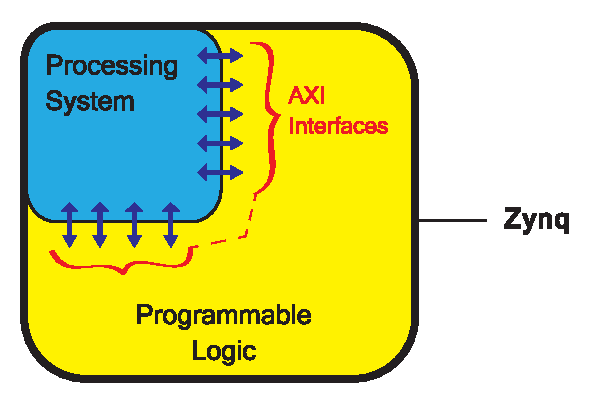
\includegraphics[width=0.6\linewidth]{Images/RevisaoDeLiteratura/ArquiteturaSimplificadaZynq.eps}
	\caption{Arquitetura Simplificada - Zynq-7000}
	\vspace{-3.5mm}
	\caption*{Fonte: \citeonline[p. 26]{zynqbook}}
	\label{fig:ArquiteturaSimplificadaZynq}
\end{figure}
\vspace{6mm}

Para entender como os componentes de um sistema digital s�o mapeados dentro de um dispositivo Zynq, e como estes s�o divididos entre o PS eo PL, � necess�rio compreender como � a arquitetura de um sistema digital comum. Para \citeonline[p. 27]{zynqbook}, o modelo b�sico do \textit{hardware} de um sistemas digitais incorpora processadores, mem�rias, barramentos de interliga��o e os mais distintos perif�ricos. Como pode ser visto na Figura (\ref{fig:ArquiteturaSimplificadaSD}).

\vspace{6mm}
\begin{figure}[H]
	\centering
	\captionsetup{width=0.6\textwidth, font=footnotesize, textfont=bf}	
	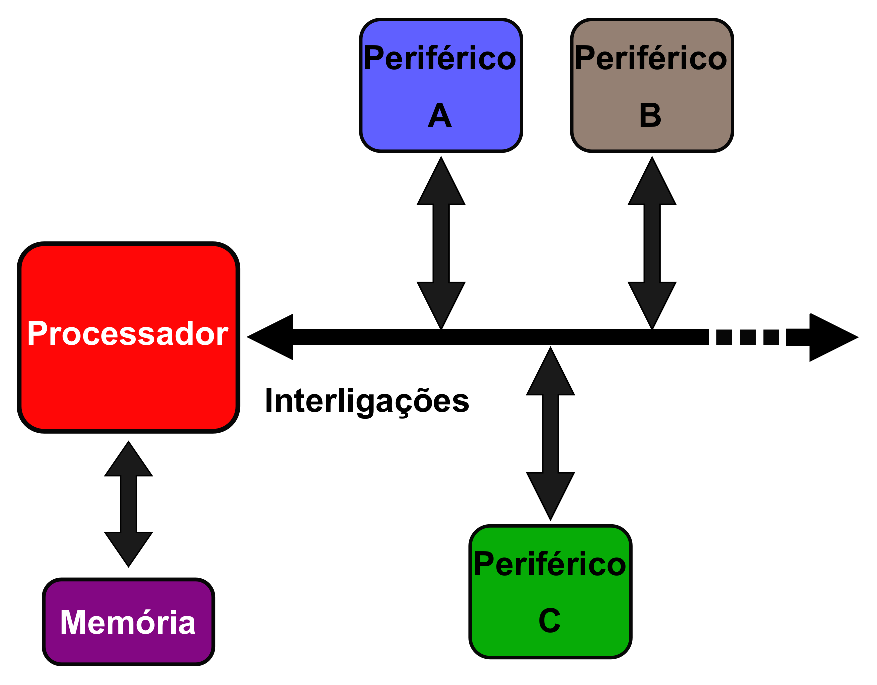
\includegraphics[width=0.6\linewidth]{Images/RevisaoDeLiteratura/ArquiteturaSimplificadaSD.eps}
	\caption{Arquitetura Simplificada de um Sistema Digital}
	\vspace{-3.5mm}
	\caption*{Fonte: \citeonline[p. 27]{zynqbook}}
	\label{fig:ArquiteturaSimplificadaSD}
\end{figure}
\vspace{6mm}

O processador � o elemento central deste modelo, pois � ele que executa o sistema de \textit{software}, que compreende as camadas de mais alto n�vel como aplica��es baseadas em sistemas operacionais, o pr�prio sistema operacional, e at� o n�vel mais baixo como o \textit{firmware} de interface com os perif�ricos do \textit{hardware}. J� os perif�ricos s�o componentes funcionais externos ao processador, e que em geral s�o divididos em tr�s tipos: 

\begin{itemize}
	
	\item \textbf{Coprocessadores :} Elementos que auxiliam o processador principal na realiza��o de tarefas especificas, geralmente projetados para otimizar tal tarefa.
	
	\item \textbf{Interfaces de Comunica��o:} Elementos respons�veis pela intera��o com interfaces externas, acionando gatilhos ou controlando portas digitais. Utilizando muitas vezes protocolos espec�ficos de comunica��o como UART ou SPI.
	
	\item \textbf{Elementos Adicionais de Mem�ria :} Elementos exclusivamente destinados ao armazenamento de dados.  
	
\end{itemize} 

A Figura (\ref{fig:ArquiteturaSimplificadaZynqSoftwareHardware}) apresentam a mesma arquitetura simplificada da Figura (\ref{fig:ArquiteturaSimplificadaSD}), por�m mapeado para um dispositivo Zynq. A estrutura do sistema digital � dividida entre processador e mem�ria para o lado PS, e os demais poss�veis perif�ricos para o lado PL. Do lado PS a arquitetura � fixa, obedecendo a estrutura definida pelo fabricando, em total contraponto com o lado PS. No lado PS a estrutura � totalmente flex�vel, limitada apenas pelo n�mero de CLBs dispon�veis da FPGA, o que oferece ao desenvolvedor um ambiente de "caixa de areia" para construir qualquer tipo de perif�rico.

\vspace{6mm}
\begin{figure}[H]
	\centering
	\captionsetup{width=0.6\textwidth, font=footnotesize, textfont=bf}	
	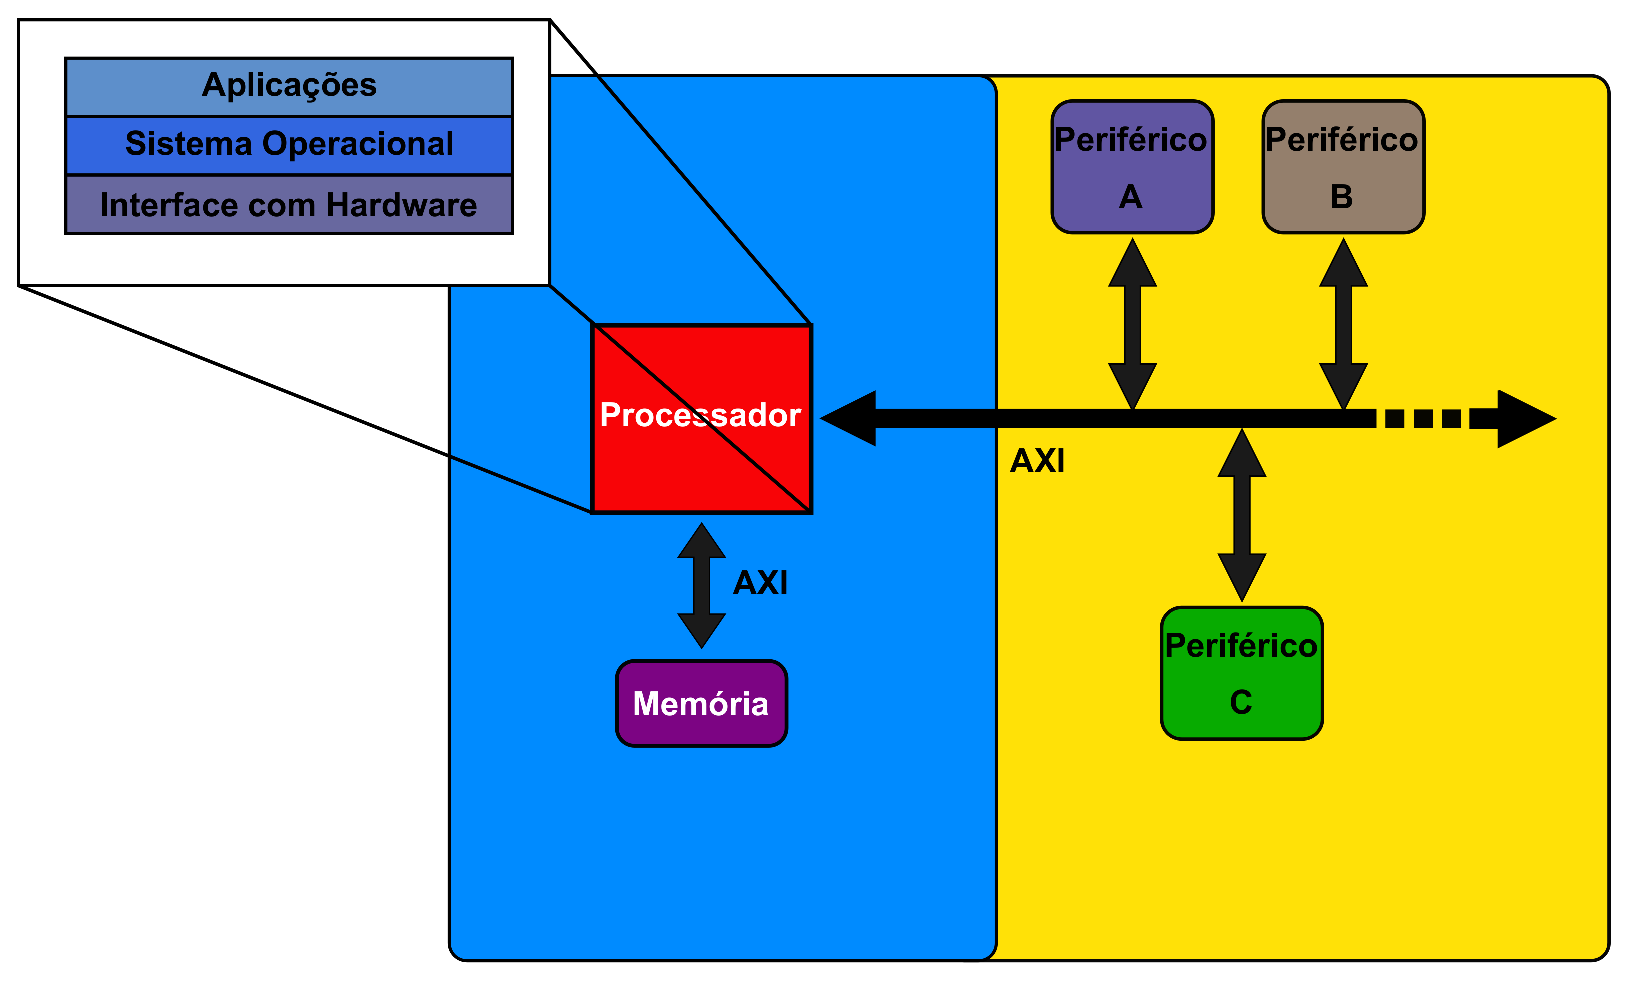
\includegraphics[width=0.6\linewidth]{Images/RevisaoDeLiteratura/ArquiteturaSimplificadaZynqSoftwareHardware.eps}
	\caption{Arquitetura Simplificado do um Sistema Digital Mapeado para o Zynq}
	\vspace{-3.5mm}
	\caption*{Fonte: \citeonline[p. 27]{zynqbook}}
	\label{fig:ArquiteturaSimplificadaZynqSoftwareHardware}
\end{figure}
\vspace{6mm}

A interface AXI possui uma grande import�ncia no desenvolvimento no Zynq-7000,j� que por meio desta interface � que os perif�ricos em PL se comunicam com o processador em PS.  A interface AXI faz parte da fam�lia de barramentos para microcontroladores ARM AMBA (\textit{Advanced Microcontroller Bus Architecture}). O ARM AMBA � um protocolo \textit{Open Standard} para conex�es e gerenciamento de blocos funcionais dentro de dispositivos  \textit{Systens-on-Chip} (Soc), facilitando o desenvolvimento de designs com m�ltiplos processadores, e com grande n�mero de controladores e perif�ricos \cite{AMBA}. A fam�lia de SoCs Zynq-7000 utilizam a interface AXI vers�o 4, o qual obedece ao mais recentes padr�es ARM AMBA 4.0 \cite{AXI}. Existem no tr�s tipos de interface AXI4:

\begin{itemize}
	
	\item \textbf{AXI :} Interface destinada a transfer�ncias de dados em alta velocidade e de maior volume utilizando mapeamento de mem�ria, utiliza endere�os de mem�ria para acessar dados e portanto consome recursos de mem�ria para ser implementado. Interface mais complexa, e oferece maiores op��es de controle de dados, inclusive transfer�ncia no modo \textit{brust}.
	
	\item \textbf{AXI-Lite:}Interface destinada a transfer�ncias de dados em baixa velocidade utilizando mapeamento de mem�ria, consome espa�o de mem�ria apenas para controlar dados da transfer�ncia, como destino, origem e status da transmiss�o. Interface mais simples do que a AXI, logo n�o oferece controle de dados como o modo \textit{brust}.
	
	\item \textbf{AXI-Stream:} Interface para transfer�ncia de dados em alta velocidade, por�m n�o utiliza mapeamento de mem�ria. Toda a transfer�ncia nesta interface � peita por em  fluxo de dados cont�nuos, os quais n�o s�o armazenados pela interface. 
	
\end{itemize} 

Dentro do ambiente do PS no Zynq al�m do processador ARM Cortex-A9  existe ainda um conjunto de perif�ricos de mem�ria, interconex�o, comunica��o e gerenciamento. A maioria destes perif�ricos utiliza a interface AXI, com 32 ou 64 Bits, inclusive a pr�prias conex�es de fronteira entre PS e PL. Diferente de PS onde a arquitetura j� est� pronta e � est�tica, em PL o desenvolvedor pode criar todo uma gama de perif�ricos, e consequentemente conecta-los com uma quantidade enorme de interfaces AXI de qualquer tipo dos j� citados. Por�m a fronteira entre PS e PL � limitada e representa um gargalo na intera��o entre os dois lados. Os dispositivos da fam�lia Zynq-7000 possuem 2 interfaces AXI Mestre de 32-Bits, 2 interfaces AXI Escravo de 32-Bits e 4 interfaces 64-Bit/32-Bit configur�veis de alta velocidade. A Figura (\ref{fig:VisaoGeralArquiteturaZynq7000}) apresenta uma vis�o geral da arquitetura do SoC Zynq-700, mostrando as conex�es AXI dentro de PS e tamb�m as conex�es na fronteira de PL. 

\vspace{6mm}
\begin{figure}[H]
	\centering
	\captionsetup{width=0.8\textwidth, font=footnotesize, textfont=bf}	
	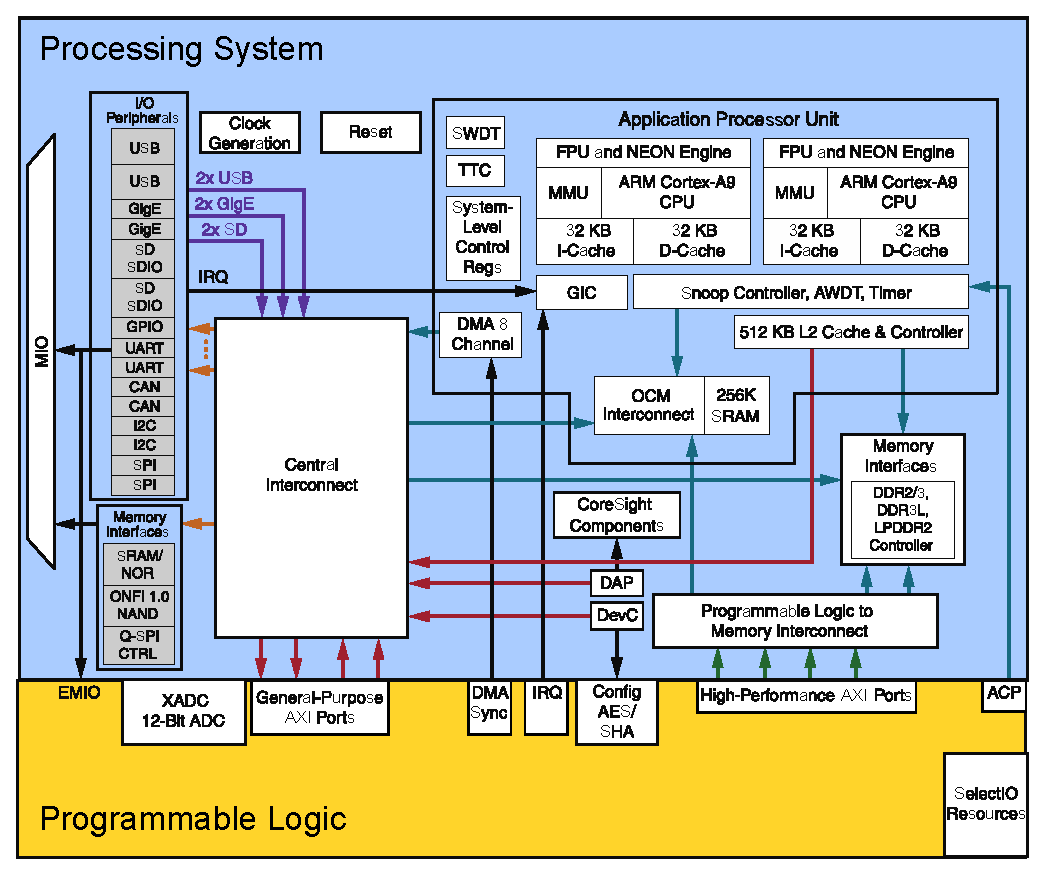
\includegraphics[width=0.8\linewidth]{Images/RevisaoDeLiteratura/VisaoGeralArquiteturaZynq7000.eps}
	\caption{Vis�o Geralda Arquitetura - Zynq 7000}
	\vspace{-3.5mm}
	\caption*{Legenda: {\color{darkgreen}AXI 32-Bits/64-Bits}, {\color{greenblue}AXI 64-Bits}, {\color{darkred}AXI 32-Bits}, {\color{palatinatepurple}AHB 32-Bits}, {\color{blackyellow}AXI 32-Bits}}
	\vspace{-3.5mm}
	\caption*{Fonte: Adaptado de \cite{zynq-7000}}
	\label{fig:VisaoGeralArquiteturaZynq7000}
\end{figure}
\vspace{6mm}



